% COMP1891 (2025/2026) - Applications in AI and Data Science
% Coursework report. Marked anonymously: do not add name, student ID or any
% other identifying detail to this file.
%
% Build:  pdflatex report.tex   (run twice for references/TOC)
% Figures are read from the parent directory, where the notebook writes them.

\documentclass[11pt,a4paper]{article}

\usepackage[margin=2.5cm]{geometry}
% Palatino for text and matching maths, replacing the default Computer Modern,
% whose thin strokes read as dated. microtype tightens justification.
\usepackage[T1]{fontenc}
\usepackage{tgpagella}
\usepackage[sc]{mathpazo}
\usepackage{courier}          % monospace that pairs with Palatino
\usepackage{microtype}
\linespread{1.05}
\usepackage{graphicx}
\usepackage{booktabs}
\usepackage{amsmath}
\usepackage{caption}
\usepackage{float}
\usepackage[hidelinks]{hyperref}
\usepackage{xcolor}

\graphicspath{{../figures/}{../}{./}}
\captionsetup{font=small,labelfont=bf}

\title{\vspace{-1.5cm}\textbf{Applications in AI and Data Science}\\[0.3em]
\large Coursework Report: Property Price Analytics and Facial Expression Detection}
\author{COMP1891 (2025/2026)\\[0.2em]
\small Module Leader: Dr Nageena Frost\\[0.15em]
\small Course Instructor: Tran-Ngoc-tran Le}
\date{Student ID: GCS240020}

\begin{document}
\maketitle

\begin{center}
\fbox{\parbox{0.93\textwidth}{\small
\textbf{Supporting code.} Every figure, table and numerical result in this report is produced by
the accompanying notebook, \texttt{COMP1891\_notebook.ipynb}, submitted alongside this document.
The notebook's cell headings match the section numbers used here (A1--A3, B1--B4, C1--C2), so
each result can be traced to the code that generated it: for example Table~\ref{tab:svm} comes
from cell B3.1 and Figure~\ref{fig:resid} from cell B1.4. The notebook is also published at
\url{https://github.com/ryanthemechanic/GRE-Coursework/blob/main/Year-2/Semester-2/COMP1891/COMP1891_notebook.ipynb}
}}
\end{center}

\vspace{0.6em}
\tableofcontents
\vspace{0.5em}
\hrule

% =====================================================================
\section{Section A: Data Science (Scenario 1)}

\subsection{A1 -- Exploratory Data Analysis}

The supplied file \texttt{Estate\_Agent.csv} contains 350 records and nine columns. It is
semicolon-delimited, so the loader detects the separator from the header line rather than
assuming a comma; read wrongly, the file collapses into a single unusable column.

The columns divide into three roles. \texttt{House\_Price} is the regression target,
\texttt{Rating} the classification target in Section B, and the remaining seven --
\texttt{House\_Area}, \texttt{Build} (year of construction), \texttt{No\_of\_Bathrooms},
\texttt{No\_of\_Bedrooms}, \texttt{Garage\_Area}, \texttt{Living\_Space} and
\texttt{Parking} -- are predictors describing the physical property.

All seven predictors are retained, on two tests: does the feature describe the property, and
does it carry signal? Table~\ref{tab:corr} shows every predictor correlating with price at
$|r| \geq 0.15$, and none is a proxy for a protected characteristic -- there is no postcode,
neighbourhood or demographic column, which materially reduces the discrimination risk
discussed in Section D. \texttt{Rating} is deliberately excluded: it correlates with price at
$r = -0.045$, and is a subjective assessment rather than a physical measurement, so including
it would make the model depend on a human judgement the agency wants to benchmark.

\begin{table}[H]
\centering
\small
\caption{Pearson correlation with \texttt{House\_Price} (after cleaning).}
\label{tab:corr}
\begin{tabular}{lc}
\toprule
\textbf{Feature} & \textbf{$r$ with House\_Price} \\
\midrule
Parking            & 0.691 \\
Garage\_Area       & 0.680 \\
Living\_Space      & 0.608 \\
No\_of\_Bathrooms  & 0.531 \\
Build              & 0.531 \\
House\_Area        & 0.286 \\
No\_of\_Bedrooms   & 0.156 \\
Rating             & $-0.045$ \\
\bottomrule
\end{tabular}
\end{table}

The strongest predictor is \texttt{Parking} ($r=0.691$), narrowly ahead of
\texttt{Garage\_Area} ($r=0.680$). Both measure the same underlying attribute -- garage
capacity as a count and as an area -- and are strongly correlated with each other, which
matters for interpreting the regression coefficients in Section B1.

The most commercially significant finding is the near-zero correlation between \texttt{Rating}
and price: the agency's own quality grade does not predict what a property sells for. Either
the grade captures something buyers do not pay for, or it is applied inconsistently, and both
readings recommend reviewing the grading process before relying on it for pricing strategy.
Figure~\ref{fig:corr} presents the full correlation matrix.

\begin{figure}[H]
\centering
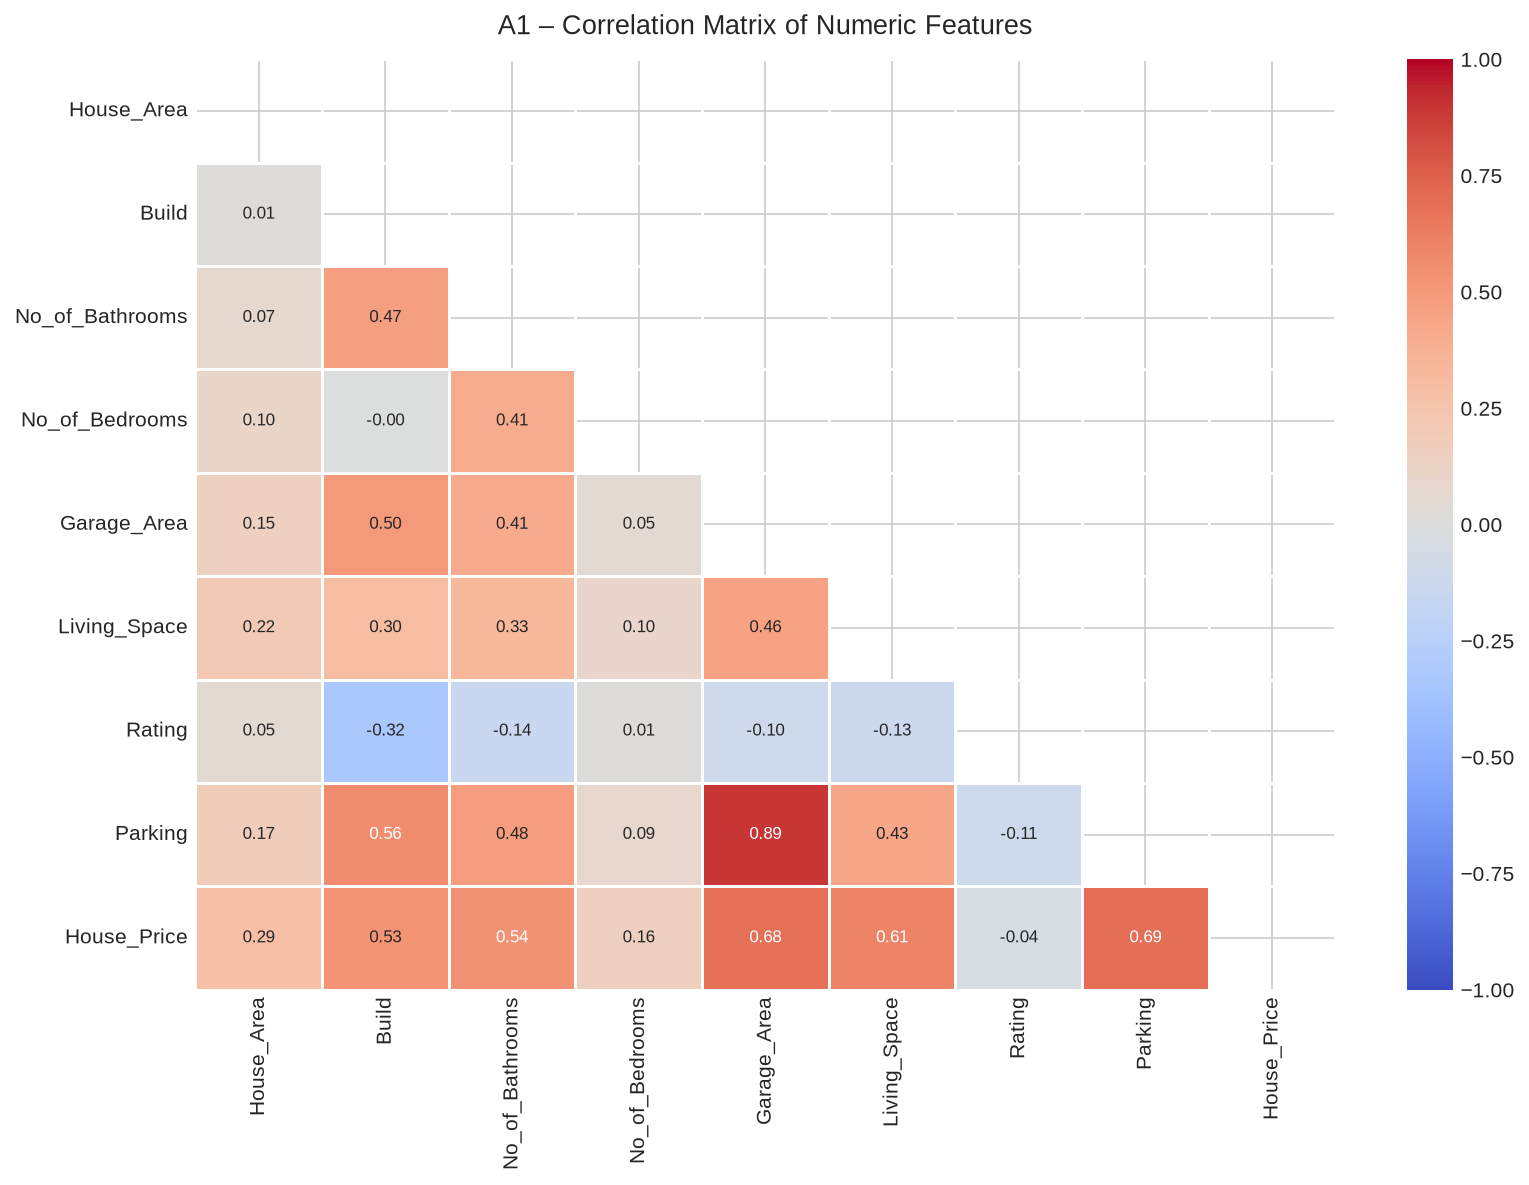
\includegraphics[width=0.78\textwidth]{A1_correlation_heatmap.png}
\caption{A1 -- Correlation matrix of all numeric features.}
\label{fig:corr}
\end{figure}

\subsection{A2 -- Data Cleaning}

The raw data is not analytics-ready. Four distinct defects were found and corrected.

\textbf{Formatting errors in a numeric column.} \texttt{Parking} is stored as text and mixes
digits with written words: nine records hold \texttt{One} (4), \texttt{Two} (3) or
\texttt{Three} (2). A naive conversion turns all nine into missing values, which median
imputation then silently overwrites with plausible-looking numbers. Since \texttt{Parking} is
the strongest price predictor, this is the most damaging defect in the file. The cleaning
routine maps written numbers to integers before conversion and reports what it changed.

\textbf{Duplicate records.} Four exact duplicates were removed (350 $\rightarrow$ 346). They
bias every statistic and can leak the same property into both training and test sets.

\textbf{Missing values.} Four columns had gaps: \texttt{Living\_Space} (5), \texttt{Garage\_Area}
(3), \texttt{No\_of\_Bathrooms} (2) and \texttt{No\_of\_Bedrooms} (2), never more than 1.4\% of
any column. Median imputation was used rather than mean because the area columns are
right-skewed, and the median is not dragged by the upper tail.

\textbf{Outliers.} Treatment was matched to each column rather than applied as one blanket rule
(Table~\ref{tab:outliers}). Price uses the conventional $1.5\times$IQR fence, excluding 14
records. The area columns are naturally right-skewed -- large plots are genuine, not erroneous
-- so the same rule would discard 17 valid properties from \texttt{House\_Area} alone. A
$3\times$IQR fence was used there, removing only the 5 implausible extremes, including one plot
of 159{,}000 square feet against a median of 9{,}378. The data falls from 346 to 327 rows.

\begin{table}[H]
\centering
\small
\caption{Outlier audit. The applied rule is shown in bold.}
\label{tab:outliers}
\begin{tabular}{lccccc}
\toprule
\textbf{Column} & \textbf{Fence} & \textbf{Lower} & \textbf{Upper} & \textbf{Outliers} & \textbf{\% of rows} \\
\midrule
House\_Price  & \textbf{1.5 IQR} & 688 & 343{,}188 & \textbf{14} & 4.0 \\
House\_Price  & 3.0 IQR & $-127{,}750$ & 471{,}625 & 2 & 0.6 \\
House\_Area   & 1.5 IQR & 1{,}603 & 17{,}569 & 17 & 4.9 \\
House\_Area   & \textbf{3.0 IQR} & $-4{,}384$ & 23{,}556 & \textbf{6} & 1.7 \\
Living\_Space & 1.5 IQR & 173 & 2{,}075 & 5 & 1.4 \\
Garage\_Area  & 1.5 IQR & $-63$ & 959 & 3 & 0.9 \\
\bottomrule
\end{tabular}
\end{table}

\begin{figure}[H]
\centering
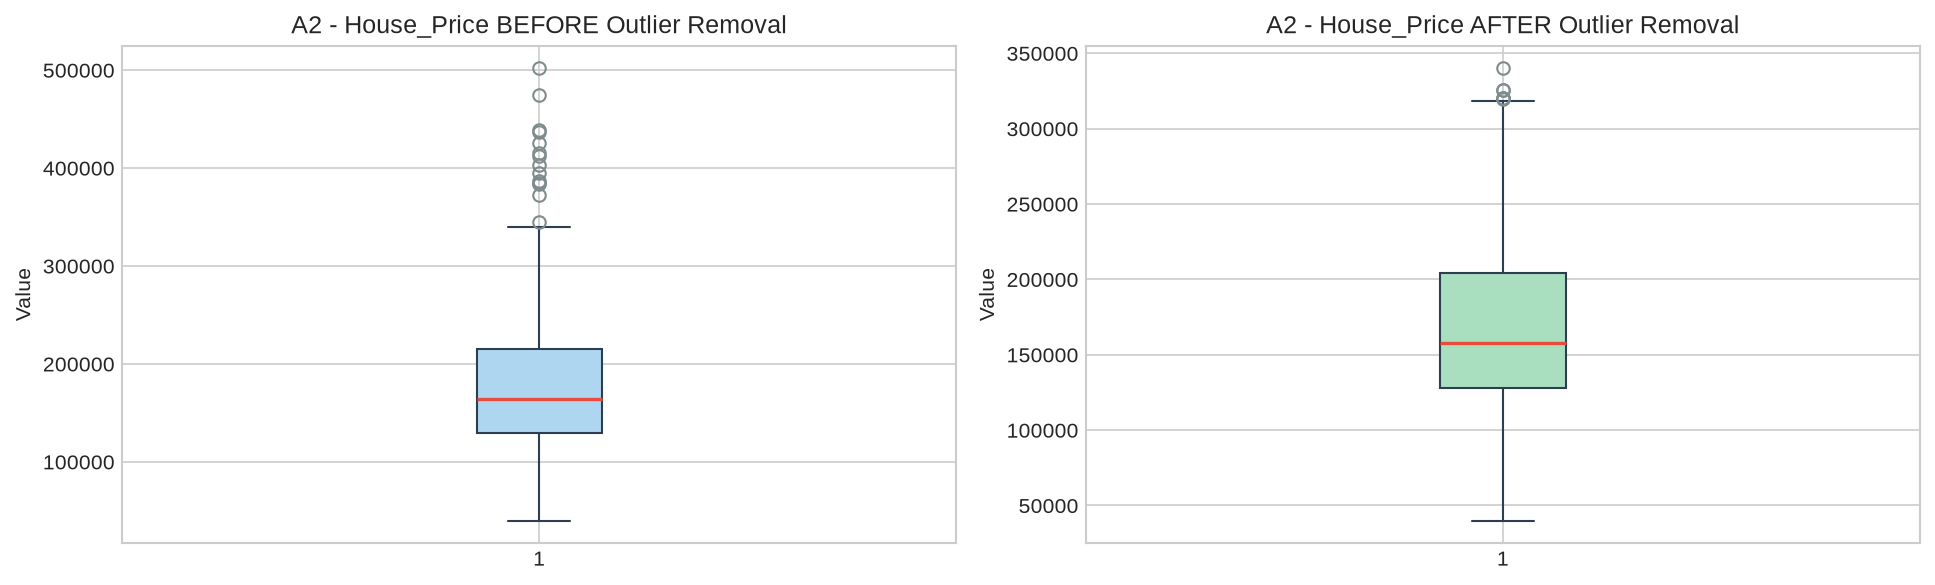
\includegraphics[width=0.85\textwidth]{A2_outlier_boxplot.png}
\caption{A2 -- Price distribution before and after outlier removal.}
\label{fig:outlier}
\end{figure}

\subsection{A3 -- Data Visualisation}

Each visualisation was chosen to answer a specific question rather than to display the data
generically.

\textbf{Price distribution (Figure~\ref{fig:price}).} Linear regression assumes normal
residuals, and a histogram with a Q--Q plot tests that directly. Post-cleaning skewness is
0.707, below the $|{\text{skew}}| > 1$ threshold for a log transformation, so price was
modelled untransformed.

\begin{figure}[H]
\centering
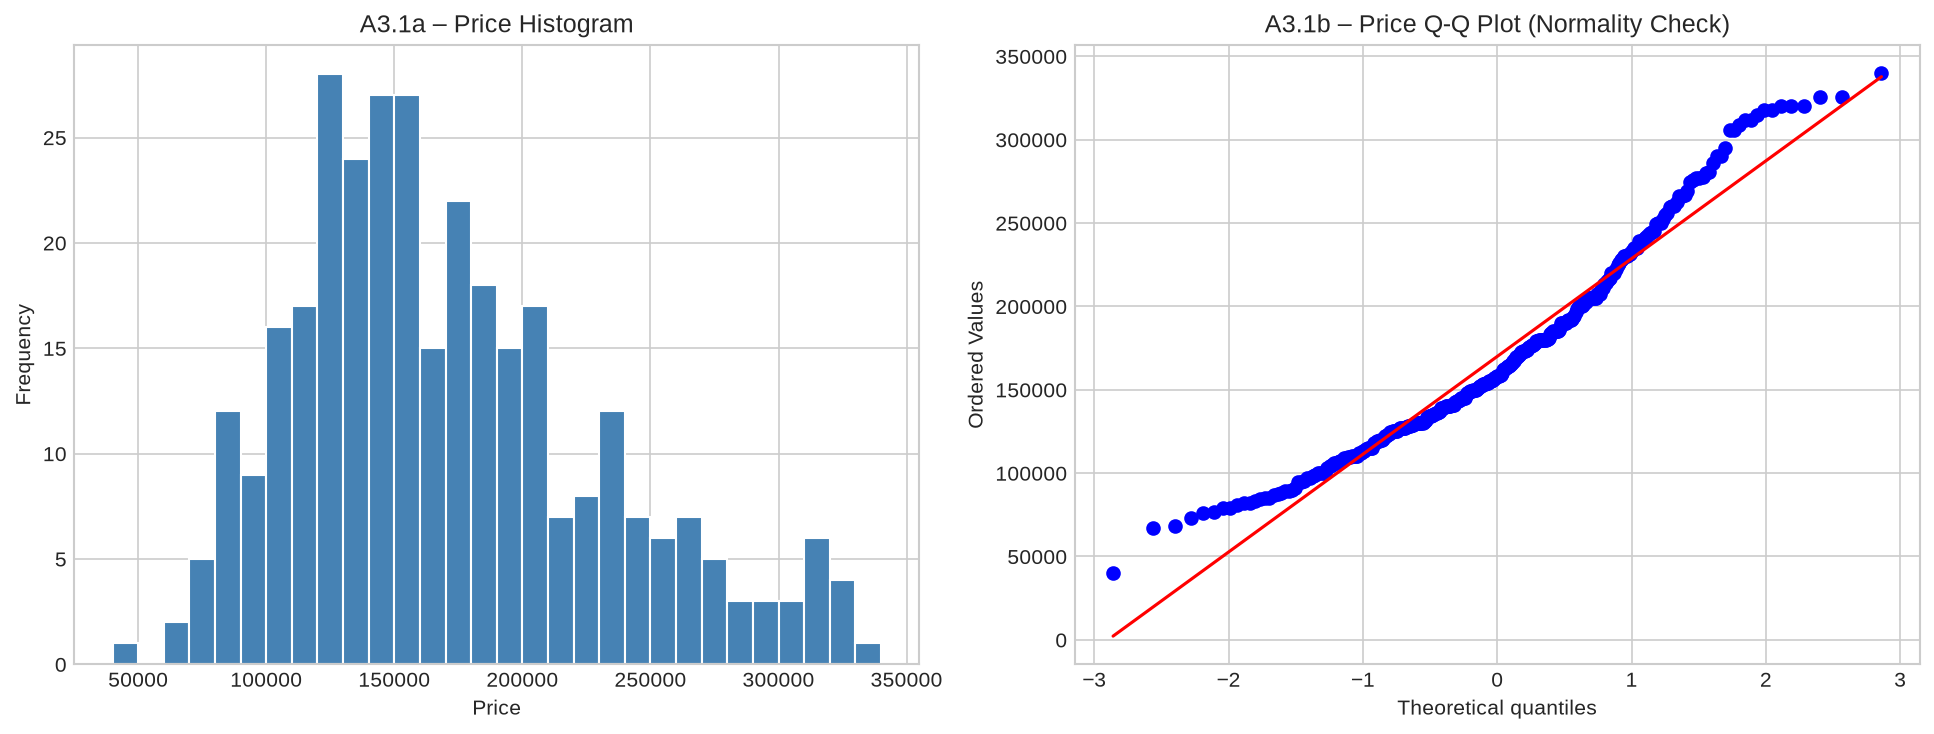
\includegraphics[width=0.85\textwidth]{A3_price_distribution.png}
\caption{A3.1 -- Price histogram and Q--Q plot.}
\label{fig:price}
\end{figure}

\textbf{Feature distributions (Figure~\ref{fig:dist}).} Count and continuous variables are
plotted differently: bedrooms, bathrooms, rating and parking take few whole-number values, so
histograms would invent fractional bins and hide category imbalance. They are drawn as category
bars annotated with the largest level's share; continuous features keep histograms.

\begin{figure}[H]
\centering
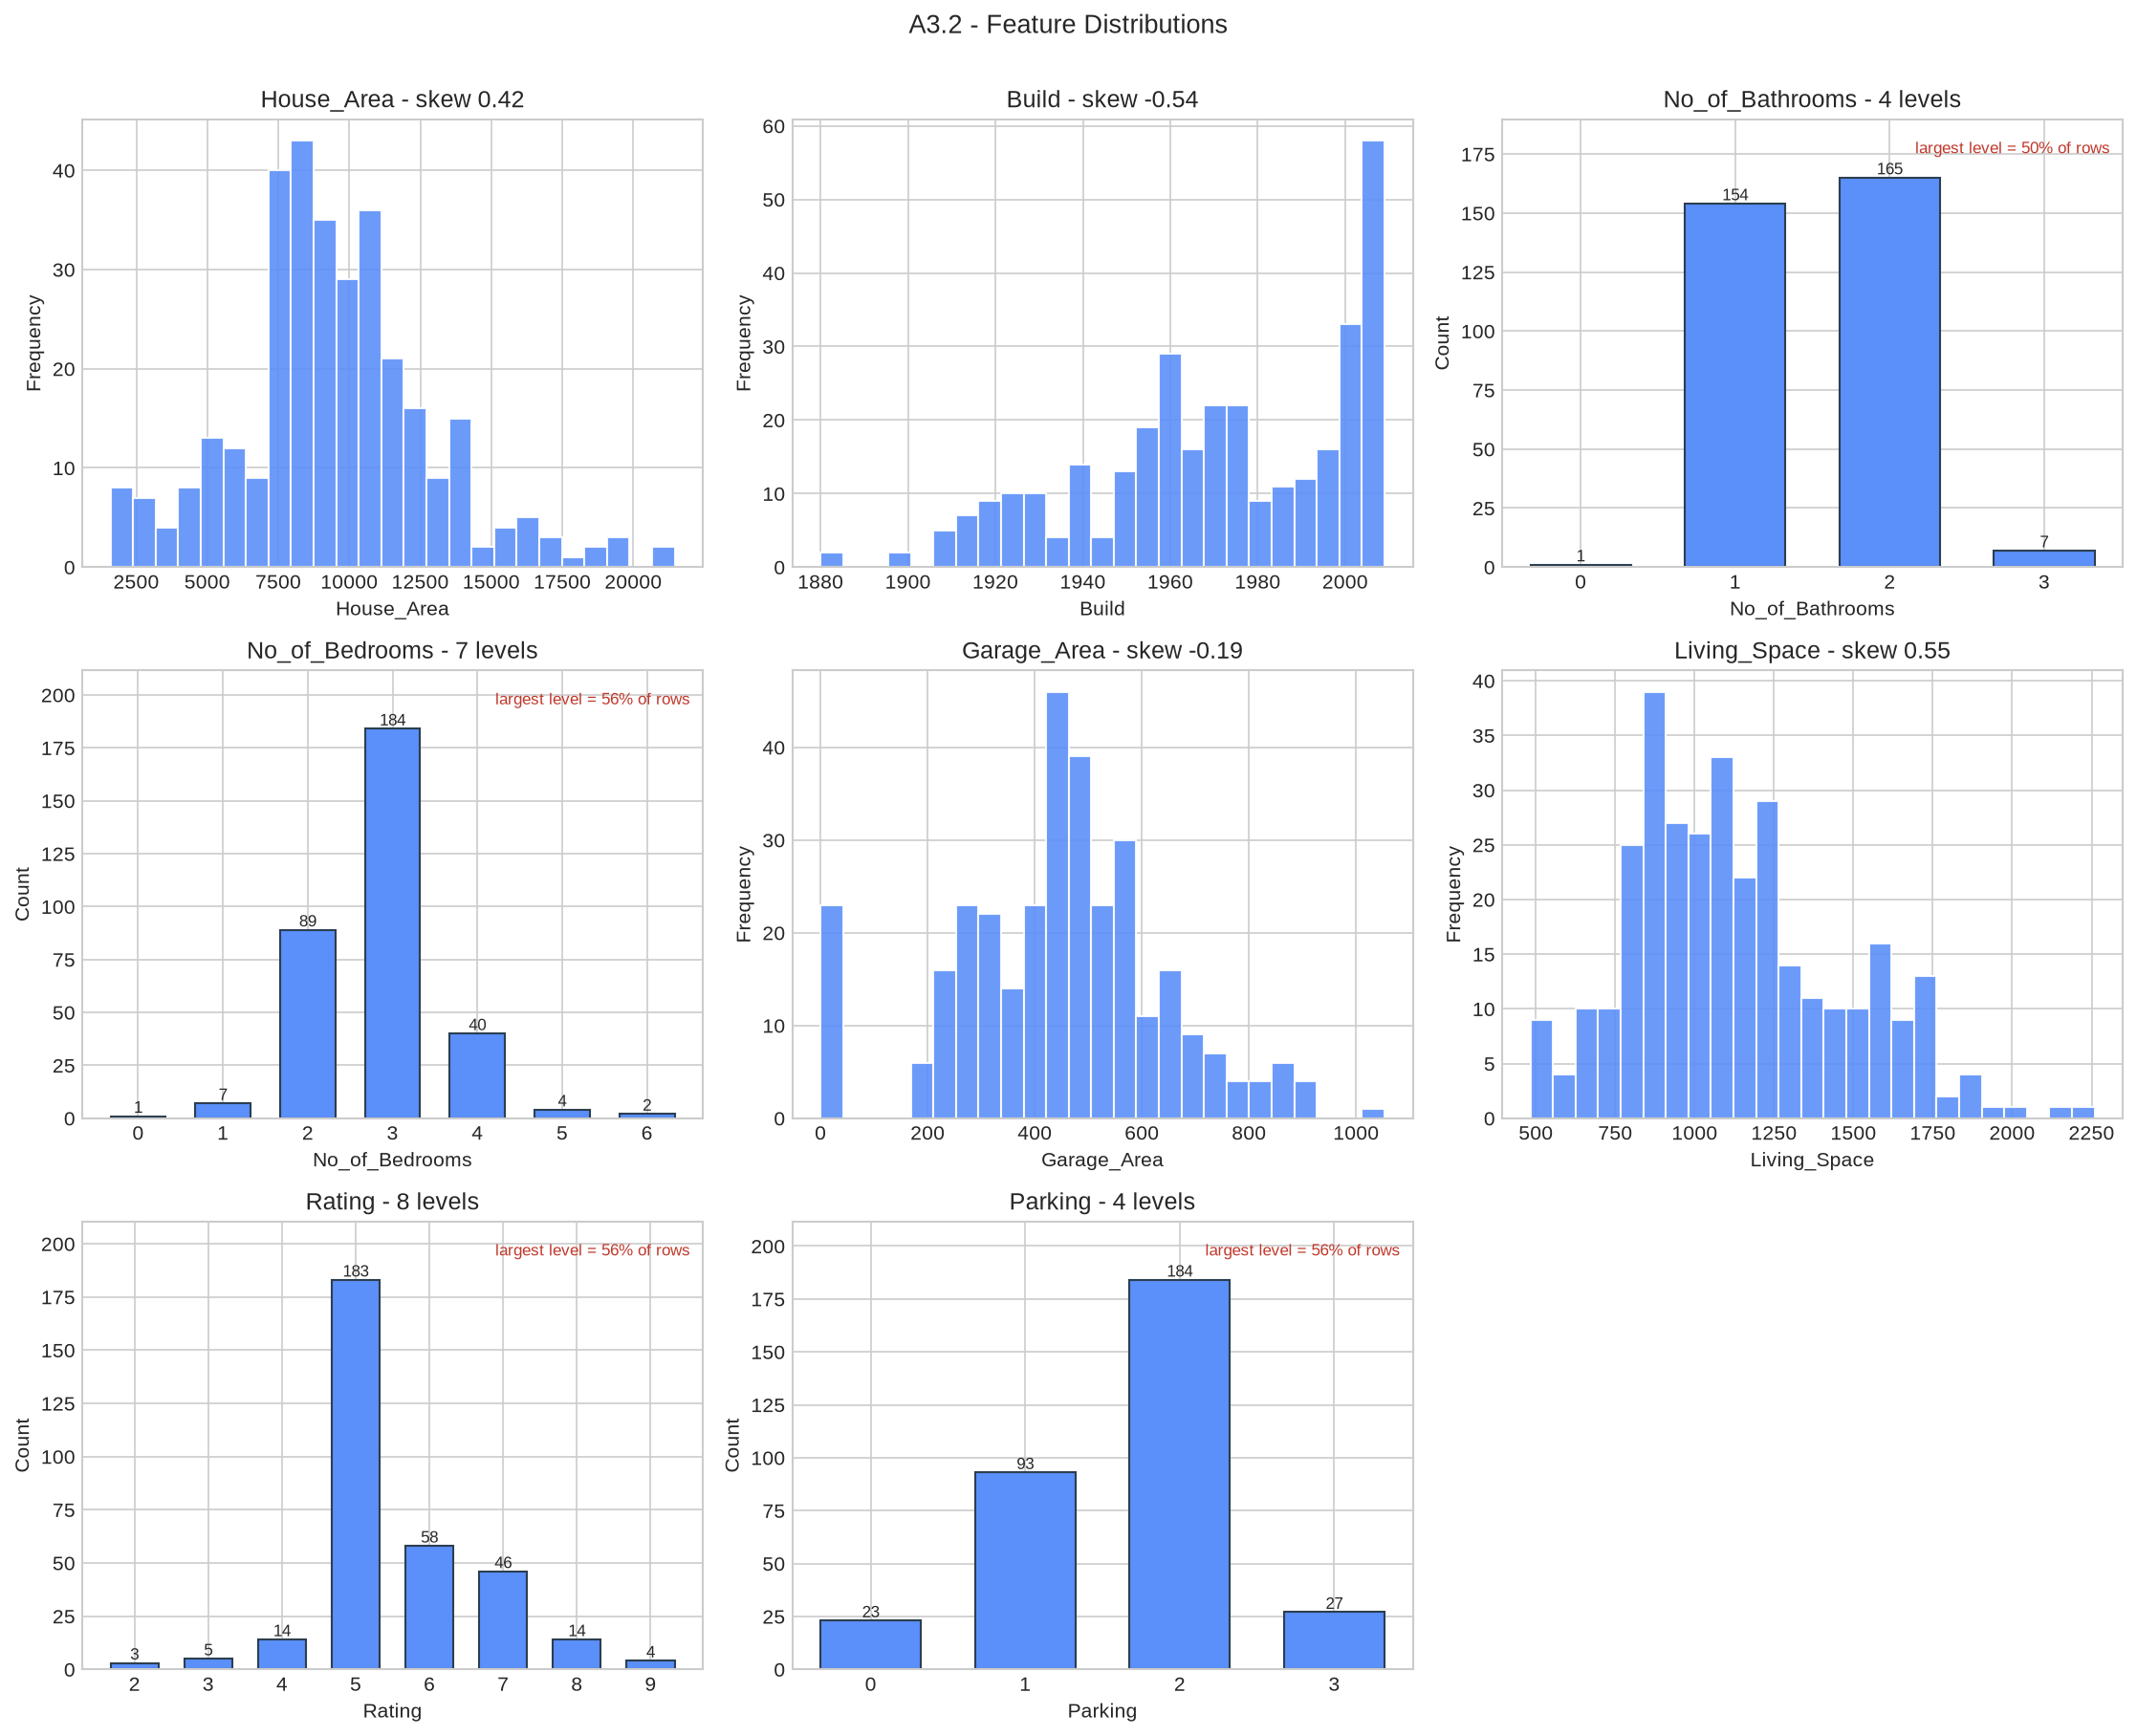
\includegraphics[width=\textwidth]{A3_feature_distributions.png}
\caption{A3.2 -- Feature distributions, split by variable type.}
\label{fig:dist}
\end{figure}

\textbf{Price against the leading predictors (Figure~\ref{fig:scatter}).} Scatter plots with a
fitted trend line test whether the correlation reflects a genuinely linear relationship, which a
single coefficient cannot distinguish from a curved one.

\begin{figure}[H]
\centering

\includegraphics[width=0.85\textwidth]{A3_scatter_price.png}
\caption{A3.3 -- Price against the two most correlated features.}
\label{fig:scatter}
\end{figure}

\textbf{Price by category (Figure~\ref{fig:box})} shows price dispersion across grades and
bedroom counts, with group sizes on the axis so a wide box resting on three properties is not
read as a pattern. It confirms visually what Table~\ref{tab:corr} states: median price does not
climb consistently with rating.

\begin{figure}[H]
\centering
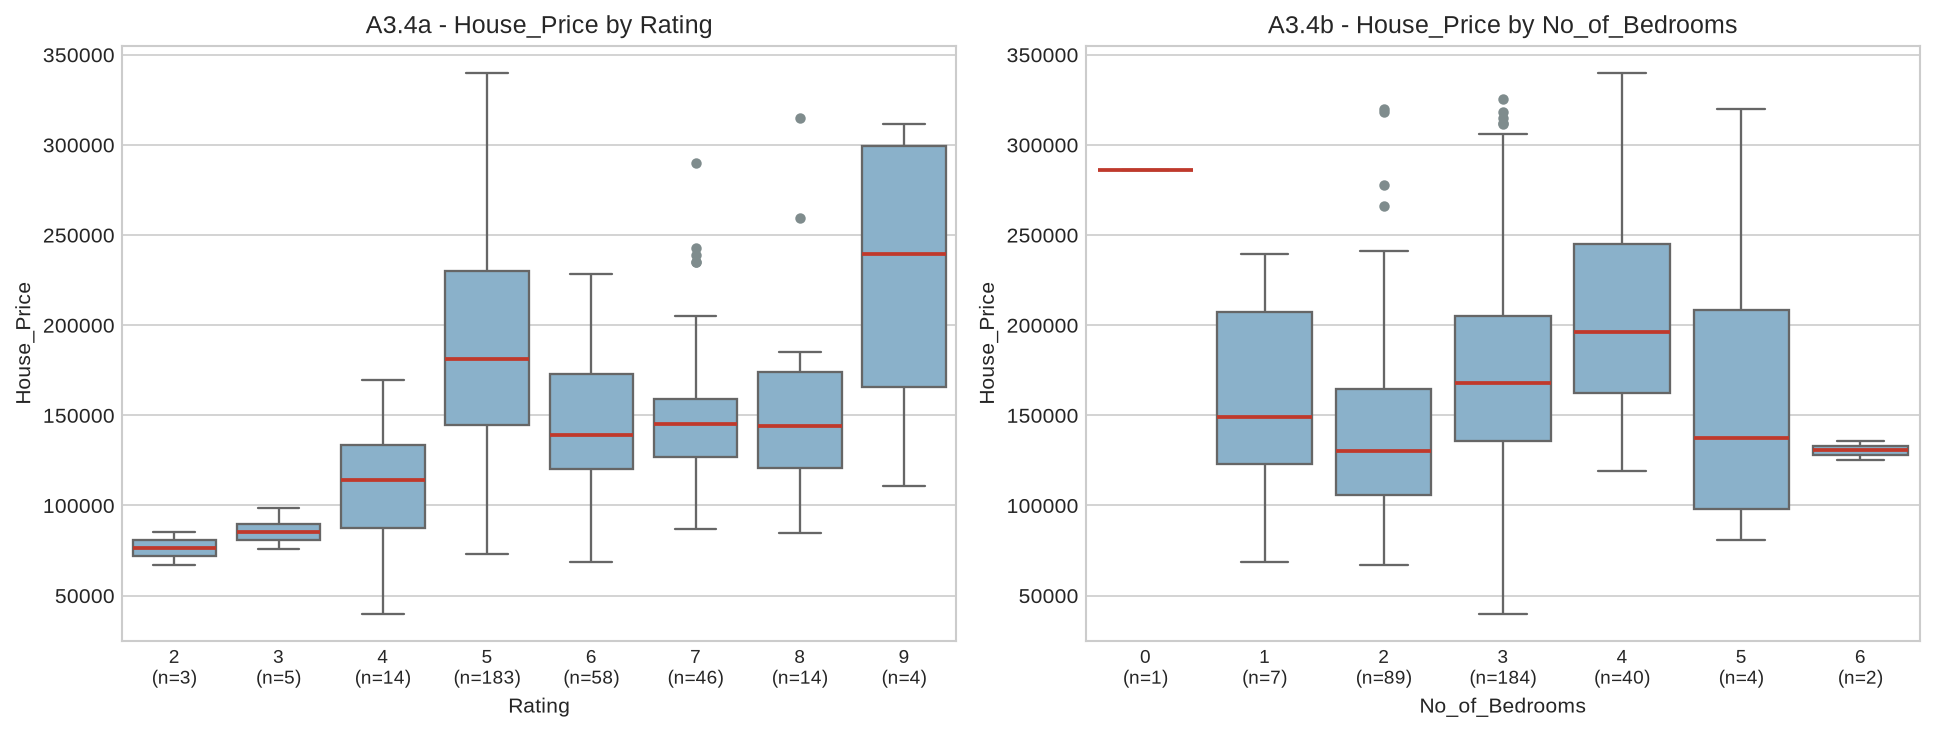
\includegraphics[width=0.85\textwidth]{A3_boxplots.png}
\caption{A3.4 -- Price by rating and by bedroom count ($n$ shown per group).}
\label{fig:box}
\end{figure}

\textbf{Class balance (Figure~\ref{fig:balance}).} \texttt{Rating} is the Section B target, so
its balance was checked before any model was fitted. Grade 5 holds 56.0\% of properties, the
imbalance ratio is 61:1, and grades 2, 3 and 9 have under ten examples each. This determines the
choice of metric throughout Section B: predicting grade 5 unconditionally already scores 56\%
accuracy while learning nothing.

\begin{figure}[H]
\centering
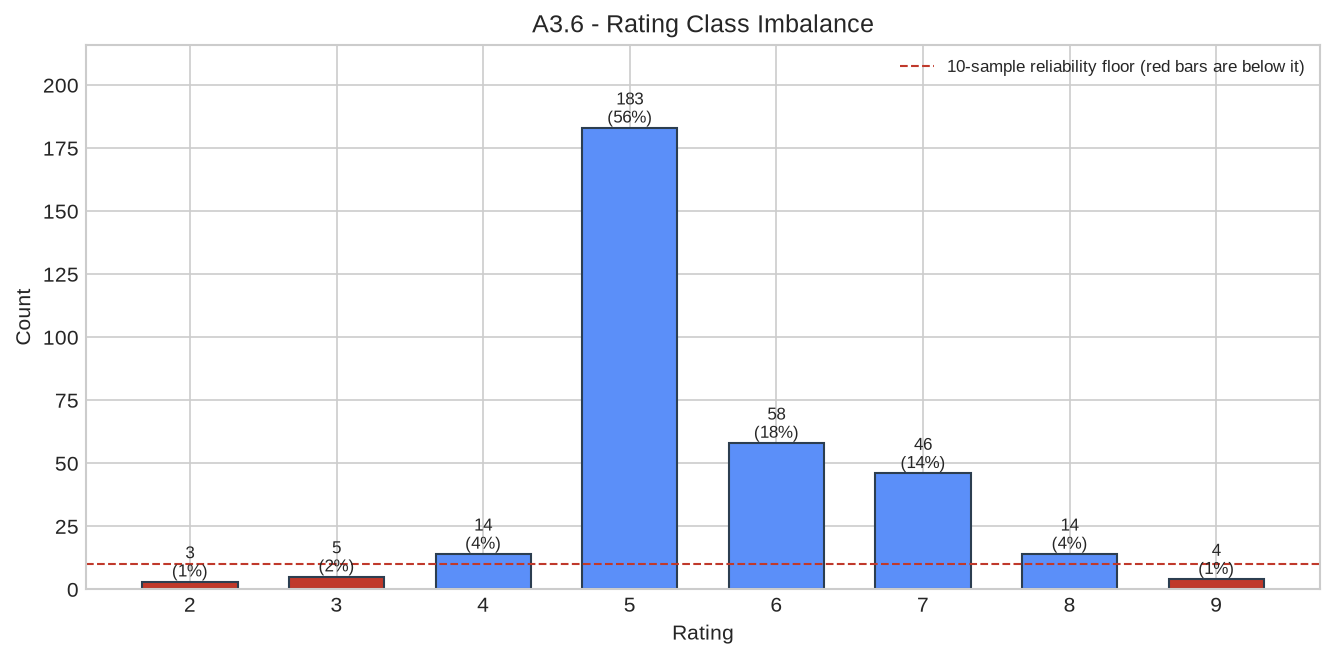
\includegraphics[width=0.72\textwidth]{A3_class_balance.png}
\caption{A3.6 -- Rating class imbalance. Red bars fall below a usable sample size.}
\label{fig:balance}
\end{figure}

% =====================================================================
\section{Section B: AI and Machine Learning (Scenario 1)}

All models are built with scikit-learn (Pedregosa \emph{et al.}, 2011), using the same seven
predictors inside a \texttt{Pipeline} of median imputation, standardisation and the estimator. Placing preprocessing in the pipeline matters: fitted once on
the full dataset, the scaler and imputer would learn the hold-out rows' statistics and leak them
into training. Measured on the banded task of B3.3, that leakage inflated cross-validated
macro-F1 from 0.469 to 0.497 and selected a different $k$. Inside a pipeline both steps refit on
each training fold alone.

\subsection{B1 -- Multiple Linear Regression}

Three train/test splits were evaluated (Table~\ref{tab:lr}). Three metrics are reported
together because each answers a different question: MAE gives the average error in pounds and
is what a client would understand; RMSE penalises large errors more heavily and so exposes
occasional bad predictions; $R^2$ states the proportion of price variance explained.

\begin{table}[H]
\centering
\small
\caption{B1 -- Linear regression across three train/test splits.}
\label{tab:lr}
\begin{tabular}{lccccc}
\toprule
\textbf{Split} & \textbf{Train} & \textbf{Test} & \textbf{MAE} & \textbf{RMSE} & \textbf{$R^2$} \\
\midrule
70/30 & 228 & 99 & 23{,}701.57 & 31{,}967.72 & 0.763 \\
80/20 & 261 & 66 & 24{,}113.45 & 31{,}915.02 & 0.763 \\
90/10 & 294 & 33 & 23{,}760.23 & 30{,}314.78 & 0.810 \\
\bottomrule
\end{tabular}
\end{table}

The reporting split was fixed at 80/20 \emph{before} any result was seen; choosing the
best-scoring split afterwards would select a model on the test set and report the flattering
0.810 from the 90/10 split, whose 33-property test set is the least reliable. On the declared
split the model explains 76.3\% of variance with a typical error of \pounds24{,}113 against a
median price near \pounds164{,}000, about 15\%.

Even that is optimistic. Five-fold cross-validation gives $R^2 = 0.637 \pm 0.148$, folds ranging
0.443 to 0.790. The single-split figures cluster near 0.76 only because they share one
convenient partition; the honest estimate is twelve points lower and far less stable. The wide
fold spread is itself a finding: with 327 records, performance depends materially on which
properties the model happens to train on.

\begin{figure}[H]
\centering

\includegraphics[width=\textwidth]{B1_regression.png}
\caption{B1 -- Predicted against actual price for each split.}
\label{fig:reg}
\end{figure}

Figure~\ref{fig:coef} shows the coefficients, but they must be read with care. Variance
inflation factors confirm the redundancy anticipated in A1: \texttt{Parking} reaches
$\mathrm{VIF} = 5.31$ and \texttt{Garage\_Area} $4.87$, so 81\% and 80\% of each is predictable
from the other features. Above the conventional threshold of 5 a coefficient is unstable,
because the model cannot separate two overlapping measurements of the same garage provision.
Predictive accuracy is unaffected -- only interpretation is. The other five features sit below
$\mathrm{VIF} = 1.8$.

Residual diagnostics (Figure~\ref{fig:resid}) test the underlying assumptions. Residuals average
near zero and are close to normal (skew 0.36), so the model is unbiased overall. But
corr(fitted, $|$residual$|$) $= 0.438$: error grows with predicted price. This heteroscedasticity
makes the model less precise on expensive properties, so the single MAE understates uncertainty
at the top of the market. High-value valuations warrant a wider interval; modelling
$\log(\text{price})$ is the standard remedy.

\begin{figure}[H]
\centering

\includegraphics[width=\textwidth]{B1_residual_diagnostics.png}
\caption{B1 -- Residual diagnostics: residuals against fitted values, their distribution, and a
normal Q--Q plot.}
\label{fig:resid}
\end{figure}

\begin{figure}[H]
\centering

\includegraphics[width=0.7\textwidth]{B1_coefficients.png}
\caption{B1 -- Standardised feature coefficients.}
\label{fig:coef}
\end{figure}

Applying the model to a median property (9{,}180 sq ft plot, built 1972, 2 bathrooms,
3 bedrooms, 454 sq ft garage, 1{,}085 sq ft living space, 2 parking spaces) predicts
\textbf{\pounds181{,}951}. Given the MAE, this should be quoted to a client as approximately
\pounds182{,}000 $\pm$ \pounds24{,}000 rather than as a point figure.

\subsection{B2 -- k-Nearest Neighbours}

$k$ was tuned across $k = 1 \ldots 25$ using stratified cross-validation on the training set
only. Selecting $k$ by test-set accuracy -- a common shortcut -- leaks the test data into model
selection and produces an optimistic score. The difference is visible here: cross-validation
selects $k = 11$, whereas $k = 7$ maximises test accuracy. Only the former is a legitimate
choice.

The extreme imbalance forces a compromise. The smallest training class holds just two
properties, capping the cross-validation at two folds -- too few for a stable estimate, which is
why the selected $k$ is itself unreliable here.

\begin{figure}[H]
\centering

\includegraphics[width=0.8\textwidth]{B2_knn_tuning.png}
\caption{B2 -- kNN tuning. Selection uses the cross-validated curve, not the test curve.}
\label{fig:knn}
\end{figure}

Cross-validation selects $k = 1$, which achieves 47.6\% accuracy -- well \emph{below} the
56.1\% majority-class baseline. Balanced accuracy is 0.163 and macro-F1 0.161. That $k=1$ wins
is itself diagnostic: on two folds of a severely imbalanced sample, no value of $k$ separates
the grades, so the search settles on the most flexible one. The per-class report confirms it --
grades 2, 3, 4, 8 and 9 all score zero on both precision and recall. Reporting only weighted F1
(0.497) would disguise this completely, which is why macro-averaged metrics are shown.

\subsection{B3 -- Support Vector Machine}

Three kernels were tuned over $C$ (and $\gamma$) by cross-validation, with
\texttt{class\_weight='balanced'} so rare grades are not discarded in favour of the dominant
one (Table~\ref{tab:svm}).

\begin{table}[H]
\centering
\small
\caption{B3 -- Tuned, class-balanced SVM by kernel.}
\label{tab:svm}
\begin{tabular}{lccccc}
\toprule
\textbf{Kernel} & \textbf{Best params} & \textbf{CV macro-F1} & \textbf{Accuracy} & \textbf{Balanced acc.} & \textbf{Macro-F1} \\
\midrule
Linear   & $C=1$                  & 0.167 & 0.476 & 0.447 & 0.257 \\
RBF      & $C=1$, $\gamma$=scale   & 0.173 & 0.512 & \textbf{0.488} & \textbf{0.333} \\
Poly (3) & $C=1$, $\gamma$=scale   & \textbf{0.180} & 0.512 & 0.315 & 0.251 \\
\bottomrule
\end{tabular}
\end{table}

Selection used cross-validated macro-F1, favouring the polynomial kernel (0.180) over RBF
(0.173); on the test set the ranking reverses (0.333 against 0.251). With two folds and rare
classes the CV estimate is itself noisy, and honouring a pre-declared rule sometimes means
reporting the model that did not win on the day.

Against kNN the SVM wins on every imbalance-aware metric: accuracy 0.512 vs 0.476, balanced
accuracy 0.315 vs 0.163, macro-F1 0.251 vs 0.161. Since the agency needs to identify unusually
high- and low-grade properties rather than restate the most common grade, the SVM is the better
model -- though neither clears the 0.561 baseline.

\begin{figure}[H]
\centering

\includegraphics[width=0.9\textwidth]{B3_comparison.png}
\caption{B3 -- kNN against SVM across four metrics, with the majority-class baseline.}
\label{fig:cmp}
\end{figure}

\textbf{Addressing the imbalance.} Neither model beats the baseline convincingly, because
grades with three to five examples cannot be learned. Grouping the eight grades into three
commercially meaningful bands -- Low ($\leq 4$, $n=22$), Mid (5--6, $n=241$) and High
($\geq 7$, $n=64$) -- keeps the business question intact while giving every class usable
support, and restores full 5-fold cross-validation. Macro-F1 rises from 0.323 to 0.503
(Table~\ref{tab:band}).

\begin{table}[H]
\centering
\small
\caption{B3.3 -- Banded rating target (baseline accuracy 0.732).}
\label{tab:band}
\begin{tabular}{lccc}
\toprule
\textbf{Model} & \textbf{Accuracy} & \textbf{Balanced acc.} & \textbf{Macro-F1} \\
\midrule
kNN ($k=5$)                       & 0.683 & 0.422 & 0.436 \\
SVM (RBF, $C=10$, $\gamma=0.1$)   & 0.634 & \textbf{0.561} & \textbf{0.503} \\
\bottomrule
\end{tabular}
\end{table}

The improvement does not come from a smarter model; it comes from asking the question at a
resolution the data can support. An estate agent advised on whether a property is a low, mid or
high grade asset is well served. A claim to separate grade 8 from grade 9 on three examples is
not defensible.

\subsubsection*{B3.4 -- Should the majority class be resampled?}

The instinct with 56\% of rows in one grade is to rebalance by resampling. That was tested
rather than assumed (Table~\ref{tab:resample}), with all resampling applied \emph{inside} each
cross-validation fold.

\begin{table}[H]
\centering
\small
\caption{B3.4 -- Imbalance treatments, SVM on the raw eight-grade target.}
\label{tab:resample}
\begin{tabular}{lcccc}
\toprule
\textbf{Treatment} & \textbf{CV macro-F1} & \textbf{Test macro-F1} & \textbf{Balanced acc.} & \textbf{Accuracy} \\
\midrule
None (baseline)             & 0.118 & 0.103 & 0.125 & 0.524 \\
\texttt{class\_weight='balanced'} & \textbf{0.173} & \textbf{0.333} & \textbf{0.488} & 0.512 \\
Random over-sampling        & 0.147 & 0.194 & 0.201 & 0.488 \\
SMOTE ($k=1$)               & \multicolumn{4}{c}{\emph{cannot run}} \\
Random under-sampling       & 0.129 & 0.104 & 0.190 & 0.305 \\
\bottomrule
\end{tabular}
\end{table}

No resampling route survives this dataset. SMOTE cannot run at all: it interpolates between a
point and its nearest same-class neighbours, but the rarest grade holds two training rows, and
inside a fold that falls to one. Under-sampling would cut training data from 245 rows to roughly
16, discarding 93\% of the evidence, and accuracy collapses to 0.305. Over-sampling merely
duplicates a few rare properties, so the model memorises those individuals. Class weighting wins
because it re-weights the loss rather than inventing or discarding data.

The counter-demonstration matters more than the table. Applying SMOTE \emph{before} the split
scores 0.801 macro-F1 against 0.333 for the best honest treatment -- but it inflates the data
from 327 to 1{,}464 rows, so most of the test set is synthetic points interpolated from the
training rows the model was fitted on. That 0.801 measures the resampling method, not the
model.

\subsection{B4 -- Clustering and Dimensionality Reduction}

$k$-means was run for $k = 2 \ldots 10$ and evaluated by the elbow method and silhouette score.
The silhouette peaks at $k = 2$ (0.287), giving two balanced segments of 161 and 166
properties -- broadly a smaller/older and a larger/newer segment.

\begin{figure}[H]
\centering

\includegraphics[width=0.85\textwidth]{B4_elbow_silhouette.png}
\caption{B4 -- Elbow and silhouette curves.}
\label{fig:elbow}
\end{figure}

Both PCA and t-SNE were applied to project the seven features into two dimensions. Rather than
asserting which performs better, both were measured (Table~\ref{tab:dr}).

\begin{table}[H]
\centering
\small
\caption{B4 -- PCA against t-SNE.}
\label{tab:dr}
\begin{tabular}{lcccc}
\toprule
\textbf{Space} & \textbf{Silhouette} & \textbf{Variance retained} & \textbf{Interpretable axes} & \textbf{Deterministic} \\
\midrule
Original (7-D) & 0.287 & 100\%   & yes & yes \\
PCA (2-D)      & 0.420 & 61.6\%  & yes & yes \\
t-SNE (2-D)    & \textbf{0.568} & n/a & no & no \\
\bottomrule
\end{tabular}
\end{table}

t-SNE produces visually tighter groups (silhouette 0.568 against 0.420), but its axes carry no
units, between-cluster distances are not meaningful, and the layout changes with the seed and
perplexity. PCA retains 61.6\% of variance in two components with axes interpretable as weighted
combinations of the original features. PCA is therefore the more appropriate estimator here,
because the agency must explain to a client \emph{why} a property falls into a segment; t-SNE
remains better for the narrower task of confirming visually that two separable segments exist.

\begin{figure}[H]
\centering

\includegraphics[width=0.49\textwidth]{B4_pca_clusters.png}
\hfill

\includegraphics[width=0.49\textwidth]{B4_tsne_clusters.png}
\caption{B4 -- Clusters under PCA (left) and t-SNE (right).}
\label{fig:dr}
\end{figure}

% =====================================================================
\section{Section C: AI -- Facial Expression Detection (Scenario 2)}

\subsection{C1 -- Detection and Measured Accuracy}

Fifty images in \texttt{FacesSample} were classified into the six expressions named in the
brief: Surprised, Angry, Happy, Sad, Frightful and Neutral. An \texttt{Expressions} folder
holding one self-selected reference image per expression was created as required. Crucially,
the sample ships with ground-truth labels (\texttt{groundtruth.json}), so detection success is
\emph{measured} rather than estimated by eye.

Two methods were implemented and compared. Both use \texttt{trpakov/vit-face-expression}, a
Vision Transformer fine-tuned on facial expressions.

\begin{itemize}
\item \textbf{Method 1 -- reference matching.} Every image is represented by its 768-dimension
CLS embedding, and each sample image takes the label of the most cosine-similar reference image.
This uses the \texttt{Expressions} folder as the task specifies, and is one-shot learning: a
single exemplar per class.
\item \textbf{Method 2 -- direct classification.} The same network's 7-way softmax head predicts
the expression directly, having been trained on thousands of labelled faces. Its \texttt{disgust}
output has no counterpart in the brief and is folded into Angry.
\end{itemize}

\begin{table}[H]
\centering
\small
\caption{C1 -- Detection accuracy against ground truth ($n = 50$).}
\label{tab:c1}
\begin{tabular}{lccc}
\toprule
\textbf{Method} & \textbf{Accuracy} & \textbf{Balanced acc.} & \textbf{Macro-F1} \\
\midrule
Random guess (6 classes)     & 0.167 & --    & --    \\
Majority class               & 0.260 & --    & --    \\
Method 1 -- reference match  & 0.660 & 0.592 & 0.570 \\
Method 2 -- ViT classifier   & \textbf{0.720} & \textbf{0.708} & \textbf{0.684} \\
\bottomrule
\end{tabular}
\end{table}

\textbf{How successful is the detection?} Both beat the 26.0\% majority-class baseline, so both
genuinely detect expression. Method 2 reaches 72.0\%; Method 1 reaches 66.0\%, strong for
learning each expression from one example, and confirming the embedding space groups faces by
expression rather than identity or lighting. The 6-point gap is the cost of one-shot learning:
an unrepresentative exemplar harms an entire category. Method 1 scores 0.00 F1 on Frightful,
failing all four such faces because its single reference does not resemble them, while Method 2
recovers them at 0.75 recall.

\textbf{Are any images wrongly detected as Neutral?} The methods fail in opposite directions.
Method 1 never wrongly assigns Neutral, but misses seven of the nine true Neutral faces --
recall of just 0.22. Method 2 wrongly labels two images Neutral, \texttt{fig109.jpg} (truly
Angry) and \texttt{fig145.jpg} (truly Sad), and misses six true Neutrals, for 0.33 recall.

Neutral is hardest for both, which is intuitive: defined by the \emph{absence} of expression, it
sits close to any weak or partial one, and a low-intensity angry or sad face is genuinely
near-neutral. This matters for the wellbeing application, where misreading distress as neutral
is the error of greatest consequence.

\begin{figure}[H]
\centering
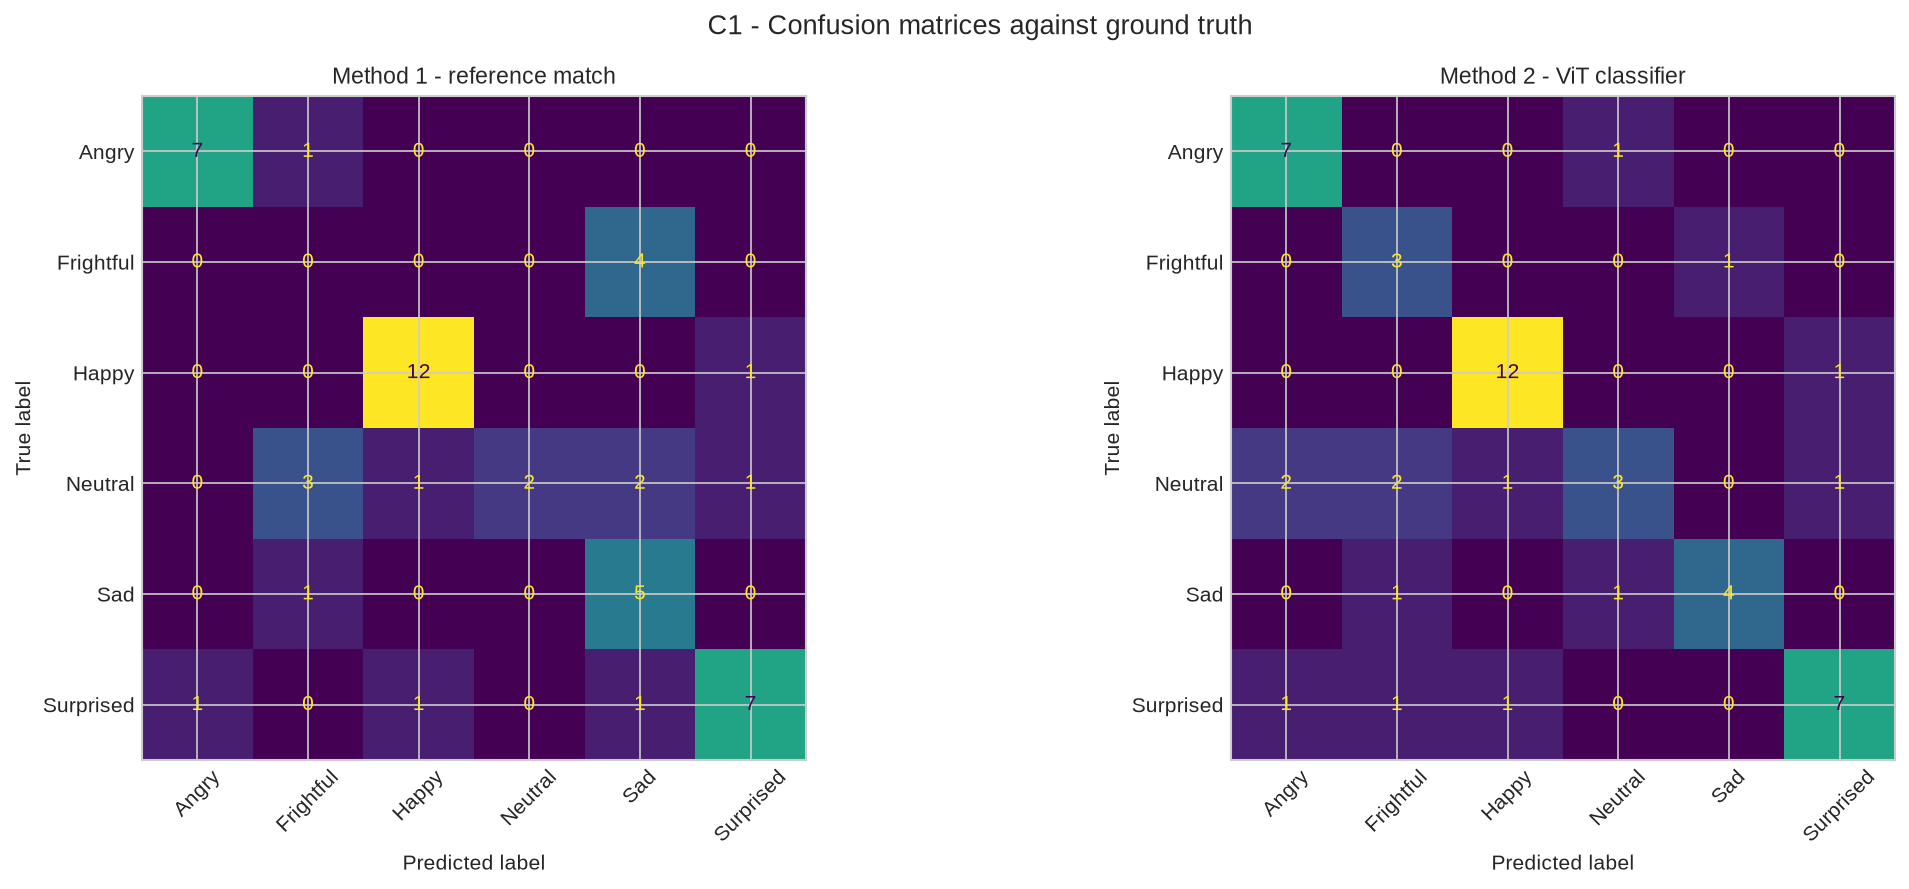
\includegraphics[width=\textwidth]{C1_confusion_matrices.png}
\caption{C1 -- Confusion matrices for both methods against ground truth.}
\label{fig:c1cm}
\end{figure}

Prediction confidence is a usable safeguard. Method 2 is 72.9\% accurate when its confidence is
at least 0.40, but only 50.0\% below it. Low-confidence predictions can therefore be routed for
human review rather than acted on automatically.

\begin{figure}[H]
\centering
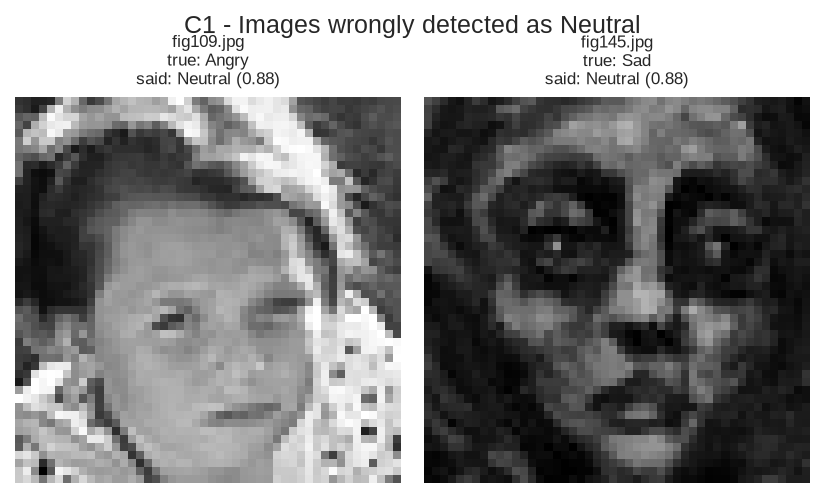
\includegraphics[width=0.9\textwidth]{C1_false_neutrals.png}
\caption{C1 -- Images wrongly detected as Neutral.}
\label{fig:neut}
\end{figure}

\subsection{C2 -- Application: Aggregated Wellbeing Monitoring}

C1 turns a face into a label. C2 models the operational system that would sit on top of it for
the corporate health and wellness initiative. Expressions are mapped to a stress weight (Happy
0.0 through Angry 0.9), averaged per employee per week over four weeks, and screened by two
rules: a \emph{level} rule (weekly mean above 0.55) and a \emph{trend} rule (a rise above 0.15
from the first week to the last).

Two rules are needed because they catch different problems: the level rule finds employees
consistently under strain, while the trend rule catches deterioration early, flagging those
whose score is still moderate but climbing. In the simulation the trend rule flags two employees
rising by 0.32 and 0.36 whom the level rule alone would have missed.

\begin{figure}[H]
\centering

\includegraphics[width=\textwidth]{C2_wellbeing_monitor.png}
\caption{C2 -- Weekly aggregated stress and trend detection.}
\label{fig:c2}
\end{figure}

The design is constrained by Section D's ethics and C1's measured accuracy. Rules operate on
weekly aggregates, never individual daily readings; managers see the team average and the number
flagged, not the per-person matrix; participation is opt-in and withdrawable. Because C1 measured
only 72\% accuracy with Neutral weakest, a flag prompts an \emph{offer} of a voluntary check-in,
never an automated intervention or any input to performance management.

% =====================================================================
\section{Section D: AI and LSEPI}

\subsection{D1 -- Legal, Social, Ethical and Professional Issues}

\textbf{Scenario 1 -- price prediction.} \emph{Legally}, property records combined with
addresses are personal data under the UK GDPR (ICO, 2021); adding postcode -- an obvious next
step -- would introduce a proxy for ethnicity and income, risking indirect discrimination under
the Equality Act 2010. \emph{Socially}, models trained on historical sales entrench inequality
by under-valuing property in deprived areas, reproducing past disadvantage as prediction
(O'Neil, 2016). \emph{Ethically}, they inherit any bias in the human valuations they learn from.
\emph{Professionally}, quoting the B1 prediction without its error margin would misrepresent its
precision, contrary to RICS transparency obligations (RICS, 2021).

\textbf{Scenario 2 -- expression monitoring.} \emph{Legally}, facial images processed to infer
mental state are biometric data engaging Article 9 of the UK GDPR, requiring explicit consent
and a Data Protection Impact Assessment (ICO, 2011). \emph{Socially}, continuous monitoring
erodes psychological safety and normalises workplace surveillance (Zuboff, 2019), and
expression norms vary across cultures and with neurodivergence, so a uniform model misreads
some groups more than others. \emph{Ethically},
employee consent may not be freely given, since refusal carries perceived career risk (Floridi
\emph{et al.}, 2018). \emph{Professionally}, presenting a 72\%-accurate classifier -- one that
misread two distressed faces as Neutral in 50 images -- as reliable would breach the ACM
requirement to assess and disclose harms (ACM, 2018).

\subsection{D2 -- Countermeasures}

For Scenario 1: complete a DPIA before deployment; exclude postcode and other protected-
characteristic proxies, as done here; publish prediction intervals with every point estimate;
apply explainable-AI methods such as SHAP; and audit periodically for disparate impact.

For Scenario 2: explicit, withdrawable consent with a penalty-free opt-out; aggregate-only
reporting, as C2 does; a human in the loop so a flag opens a conversation rather than triggering
an action; publication of the measured accuracy and weakest class; deletion of raw images once
scored; and review of error rates across demographic groups.

\subsection{D3 -- Intelligent Systems for the Common Good}

In Scenario 1, transparent pricing models can democratise market information, giving first-time
buyers analytical capability once confined to institutional investors, while aggregated signals
help local authorities identify gentrification and target affordable housing. The Rating finding
shows the wider value: data science can reveal that an established practice does not track the
outcome it claims to.

In Scenario 2, the same technology deployed with consent supports early detection of mental
health deterioration in clinical settings, and in education can identify distressed students for
pastoral support (D'Mello \emph{et al.}, 2017). What separates beneficial from harmful use is
not the algorithm but who holds the output, whether participation is voluntary, and whether the
error rate is disclosed.

% =====================================================================
\section{Section E: Conclusion and Personal Reflections}

\subsection{E1 -- Conclusion}

In Scenario 1, cleaning was where most of the value lay: nine \texttt{Parking} values stored as
words would have been silently destroyed by a naive numeric conversion, and since
\texttt{Parking} is the strongest price predictor ($r = 0.691$), that defect alone would have
degraded every downstream model. Regression explained 76.3\% of price variance on the
pre-declared split, but five-fold cross-validation put the honest figure at $0.637 \pm 0.148$:
indicative guidance, not a basis for setting an asking price.

Classifying Rating exposed the limits of the data. With grade 5 holding 56\% of records and
three grades holding under ten examples, neither kNN (0.476) nor SVM (0.512) beat the 0.561
baseline. Re-posing the task as three bands raised macro-F1 from 0.251 to 0.503 -- matching the
question to the resolution the data supports mattered more than the choice of algorithm.
Clustering found two market segments; t-SNE separated them more attractively, but PCA was
selected because only its axes can be explained to a client.

In Scenario 2, both methods beat chance: reference matching against a single exemplar reached
66.0\% accuracy, the direct classifier 72.0\%. Neutral was weakest for both, and they failed in
opposite directions -- reference matching never issued a false Neutral but missed seven of nine
true ones, while the classifier misread two distressed faces as Neutral. That error shaped the
C2 design, where aggregate reporting, dual level-and-trend rules and mandatory human review
follow from measured limitations rather than generic caution.

The overriding lesson is that the headline metric is rarely the honest one. Accuracy flattered
models that had learned only to repeat the majority class; a single split overstated $R^2$ by
twelve points; one MAE hid that error grows with price; and a bar chart of predicted expressions
would have looked plausible while concealing seven missed Neutral faces.

\subsection{E2 -- Personal Reflections}

The most instructive problems here were not the modelling steps but the points where code ran
successfully and produced wrong answers.

The clearest was the \texttt{Parking} column. My first cleaning routine converted it to numeric
without error and reported no missing values afterwards. Only when I printed what the
conversion had \emph{changed} did I find that nine values reading \texttt{One}, \texttt{Two}
and \texttt{Three} had become NaN and then been overwritten by the median. Nothing failed; the
data was simply wrong. Making cleaning routines report what they alter is now a habit, and it
caught a second defect -- the column detector searched for ``year'' and never matched
\texttt{Build}, so year of construction was silently dropped from the feature set.

Leakage taught the second lesson, twice. My initial kNN chose $k$ by test-set accuracy, which I
did not recognise as leakage until cross-validation disagreed with it. Having fixed that, I
found a subtler instance still in place: the \texttt{StandardScaler} was fitted on the whole
dataset before splitting, so every model had already seen the hold-out rows' mean and variance.
Moving preprocessing inside a \texttt{Pipeline} changed both the scores and the selected
hyperparameters. Leakage is not one mistake to check off but a category to design against, which
is what pipelines exist for. Relatedly, I first judged the classifiers on accuracy and concluded
kNN was better, until macro-F1 showed it scoring 0.00 on five of the eight grades: choosing a
metric is a modelling decision, not a reporting formality.

A third came from my own C2 simulation. I wrote the expression-probability weights as a
positional list, but the labels were sorted alphabetically, so the ``calm'' weight landed on
Angry and the stress model ran backwards -- employees scripted to deteriorate appeared to
improve, with entirely plausible-looking output. Keying the weights by name removed the whole
class of bug, teaching me to prefer constructs in which the mistake cannot be expressed.

Technically I gained fluency in pandas, in scikit-learn pipelines, and in applying pre-trained
transformers through Hugging Face, including extracting intermediate embeddings for one-shot
matching rather than only using the classification head. Dependency management proved as
consequential as modelling: DeepFace required TensorFlow, which had no build for my Python
version, so I moved to a PyTorch-only Vision Transformer. Above all I learned scepticism about
my own results, and the habit I am taking forward is checking every plausible answer against a
baseline -- because a model producing sensible-looking numbers while learning nothing is more
dangerous than one that visibly fails.

% =====================================================================
\section*{References}
\addcontentsline{toc}{section}{References}

\begin{description}
\item ACM (2018) \emph{ACM Code of Ethics and Professional Conduct}. Available at:
\url{https://www.acm.org/code-of-ethics} (Accessed: 10 August 2026).
\item D'Mello, S.K., Dieterle, E. and Duckworth, A. (2017) `Advanced, analytic, automated (AAA)
measurement of engagement during learning', \emph{Educational Psychologist}, 52(2), pp.~104--123.

\item Floridi, L., Cowls, J., Beltrametti, M., Chatila, R., Chazerand, P., Dignum, V., Luetge,
C., Madelin, R., Pagallo, U., Rossi, F., Schafer, B., Valcke, P. and Vayena, E. (2018)
`AI4People -- an ethical framework for a good AI society: opportunities, risks, principles, and
recommendations', \emph{Minds and Machines}, 28(4), pp.~689--707.
\item ICO (2011) \emph{The Employment Practices Code}. Wilmslow: Information Commissioner's
Office.
\item ICO (2021) \emph{Guide to the UK General Data Protection Regulation}. Wilmslow:
Information Commissioner's Office. Available at:
\url{https://ico.org.uk/for-organisations/uk-gdpr-guidance-and-resources/}
(Accessed: 11 August 2026).
\item O'Neil, C. (2016) \emph{Weapons of Math Destruction: How Big Data Increases Inequality and
Threatens Democracy}. New York: Crown Publishers.
\item Pedregosa, F., Varoquaux, G., Gramfort, A. \emph{et al.} (2011) `Scikit-learn: machine
learning in Python', \emph{Journal of Machine Learning Research}, 12, pp.~2825--2830.
\item RICS (2021) \emph{RICS Valuation -- Global Standards}. London: Royal Institution of
Chartered Surveyors.
\item Zuboff, S. (2019) \emph{The Age of Surveillance Capitalism}. London: Profile Books.
\end{description}

\end{document}
